\chapter{Solutions of Non-regular Point}
\label{cha:result}




\section{Overdetermined System}
\subsection{Least-Squared Method}


\subsection{Conjugate Gradient and Preconditioning}

\section{Rank Deficiency}
\subsection{Orthogonal Matching Pursuit Algorithm}
In a linear system $Ax=b$, if $A$ is rank deficient, there are two problems. The first problem is that there is not be an exact solution at all. Since the range of $A$ does not span the entire $\mathbb{R}^n$ (if $A$ has $n$ columns) but only an $(N-1)$-dimensional subspace. In this case, we can solve exactly for $x$ only if $b$ is in this subspace. The second problem is that there are actually infinity solutions, since $A$ has a non-empty null space, which means that there is a 1-dimensional subspace of vectors $x$ that gives $Ax=0$. 


\subsection{Strategies in Applications}

\section{Non-convex Problems}
\subsection{Augumented Lagrange Method}
\subsection{Non-linear Lagrangian Duality}


% \begin{figure*}
%   \label{fig:cost}
%   \subfigure[Fraction of cycles spent on zeroing\label{fig:zerocost}]{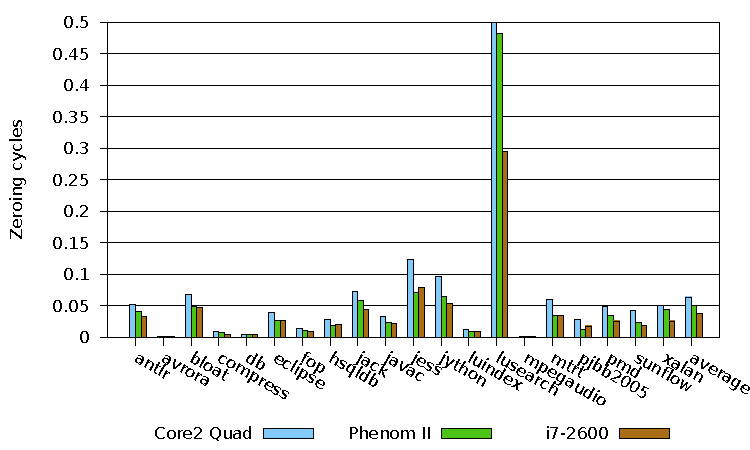
\includegraphics[width=\columnwidth]{figs/zerocost_intel.pdf}}
%   \subfigure[BytesZeroed / BytesBurstTransactionsTransferred\label{fig:zerobus}]{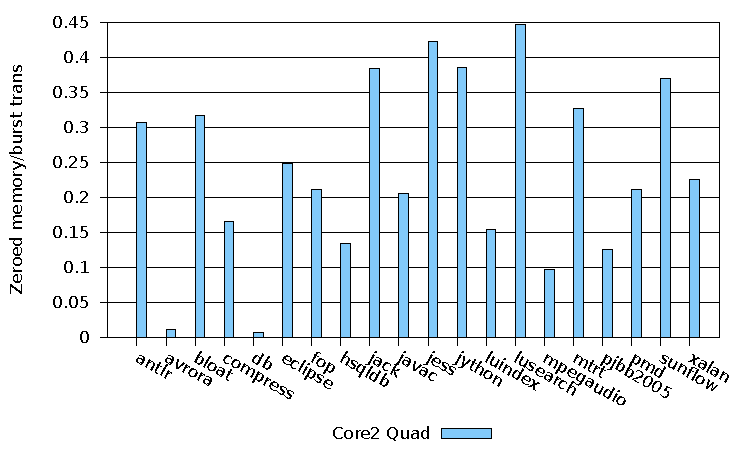
\includegraphics[width=1.0\columnwidth]{figs/zerobus_core.pdf}}
%   \caption{The cost of zero initialization}
% \end{figure*}


\section{Summary}
